\section{Overview}\label{sec:overview}

The PLoP companion, \emph{Patterns for a New Generation: AIF and Embeddings},
presents patterns for an active-inference harness: observe a coding project,
propose and score work, select an allowed action, enact it and learn from the
outcome. Its component witnesses motivated a harder question: does one
recorded attempt traverse the claimed architecture, with each output consumed
in the sense the next stage requires?

FUTON 2026 follows that question through the implementation and the operator's
working practice. It has an independent purpose: to explain how a research
apparatus can expose the difference between what it defines, what it runs and
what it demonstrates. The separate mathematical companion supplies formal
background; neither companion substitutes for a run of the integrated system.

\begin{figure}
  \centering
  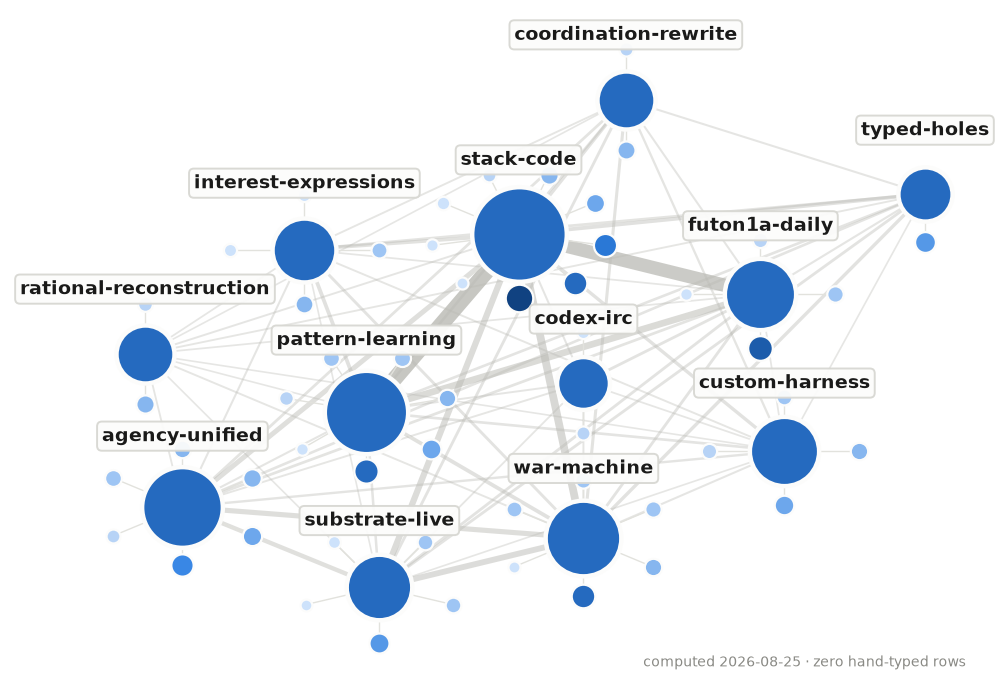
\includegraphics{feature-constellation-margin}
  \caption{A projection of recorded work. Missions occupy embedding coordinates;
  magnitude combines applied pattern warrants and incident road attestation.
  The $k{=}1$ retraction retains nodes strictly above the median magnitude,
  edges between survivors and the largest component. It shows where evidence
  accumulated, not whether the missions achieved their intended effects.}
  \label{fig:constellation}
\end{figure}

The stack contains both execution machinery---dispatch, transport, persistence
and retrieval---and records that describe it: missions, contracts, diagrams and
run receipts. The latter make an audit possible but can be stale or wrong.
For example, \texttt{M-transport-adapters} recorded a subsystem with passing
tests but no HTTP or WebSocket boundary; \texttt{M-codex-irc-execution} named
completion prose without execution evidence. Such problem statements are
useful because they identify a behaviour that a later test can attempt to
refute. A capability map alone cannot do that.

Three questions organise the paper:
\begin{enumerate}
\item Which declared constraints govern the implementation, and where does
      execution fail to satisfy them?
\item What evidence connects a proposal, its enactment and an outcome,
      including the operator's response?
\item What further evidence would justify using this apparatus beyond the
      project that built it?
\end{enumerate}

The audit case and issue board precede the detailed argument. Part~I relates
war-room constraints to mechanisms. Part~II examines operator traces and the
limits of interpreting them. Part~III describes an unrun transfer study.
Part~IV separates maintained observations, proposed attribution and preferences
over outcomes. The Snatch appendix supplies a bounded experiment, not a
substitute for War Machine validation.

Current status belongs to the generated issue board, whose records carry their
source dates. Dates in the narrative identify historical observations.
R-identifiers also retain their source scheme: the control-map registry and
PLoP catalogue are not interchangeable numbering systems. A shared number is
not a join key without the corresponding mechanism definition.
